\chapter[Models]{Physical and numerical models}

\section{Physical and mathematical description} 

Characteristic of compositional multiphase models is that the phases
are not only matter of a single chemical substance. Instead, their
composition in general includes several species, and for the mass transfer, 
the component behavior is quite different from the phase behavior. In the following, we
give some basic definitions and assumptions that are required for the
formulation of the model concept below. As an example, we take a
three-phase three-component system water-NAPL-gas
\cite{A3:class:2002a}. The modification for other multicomponent
systems is straightforward and can be found, e.\ g., in
\cite{A3:bielinski:2006,A3:acosta:2006}.

\subsection{Basic Definitions and Assumptions for the Compositional
  Model Concept}
\textbf{Components:}
The term \emph{component} stands for constituents of the phases which
can be associated with a unique chemical species, or, more generally, with 
a group of species exploiting similar physical behavior. In this work, we
assume a water-gas-NAPL system composed of the phases water (subscript
$\text{w}$), gas ($\text{g}$), and NAPL ($\text{n}$). These phases are
composed of the components water (superscript $\text{w}$), air
($\text{a}$), and the organic contaminant ($\text{c}$) (see Fig.\
\ref{A3:fig:mundwtrans}).
%
\begin{figure}[hbt]
  \centering
  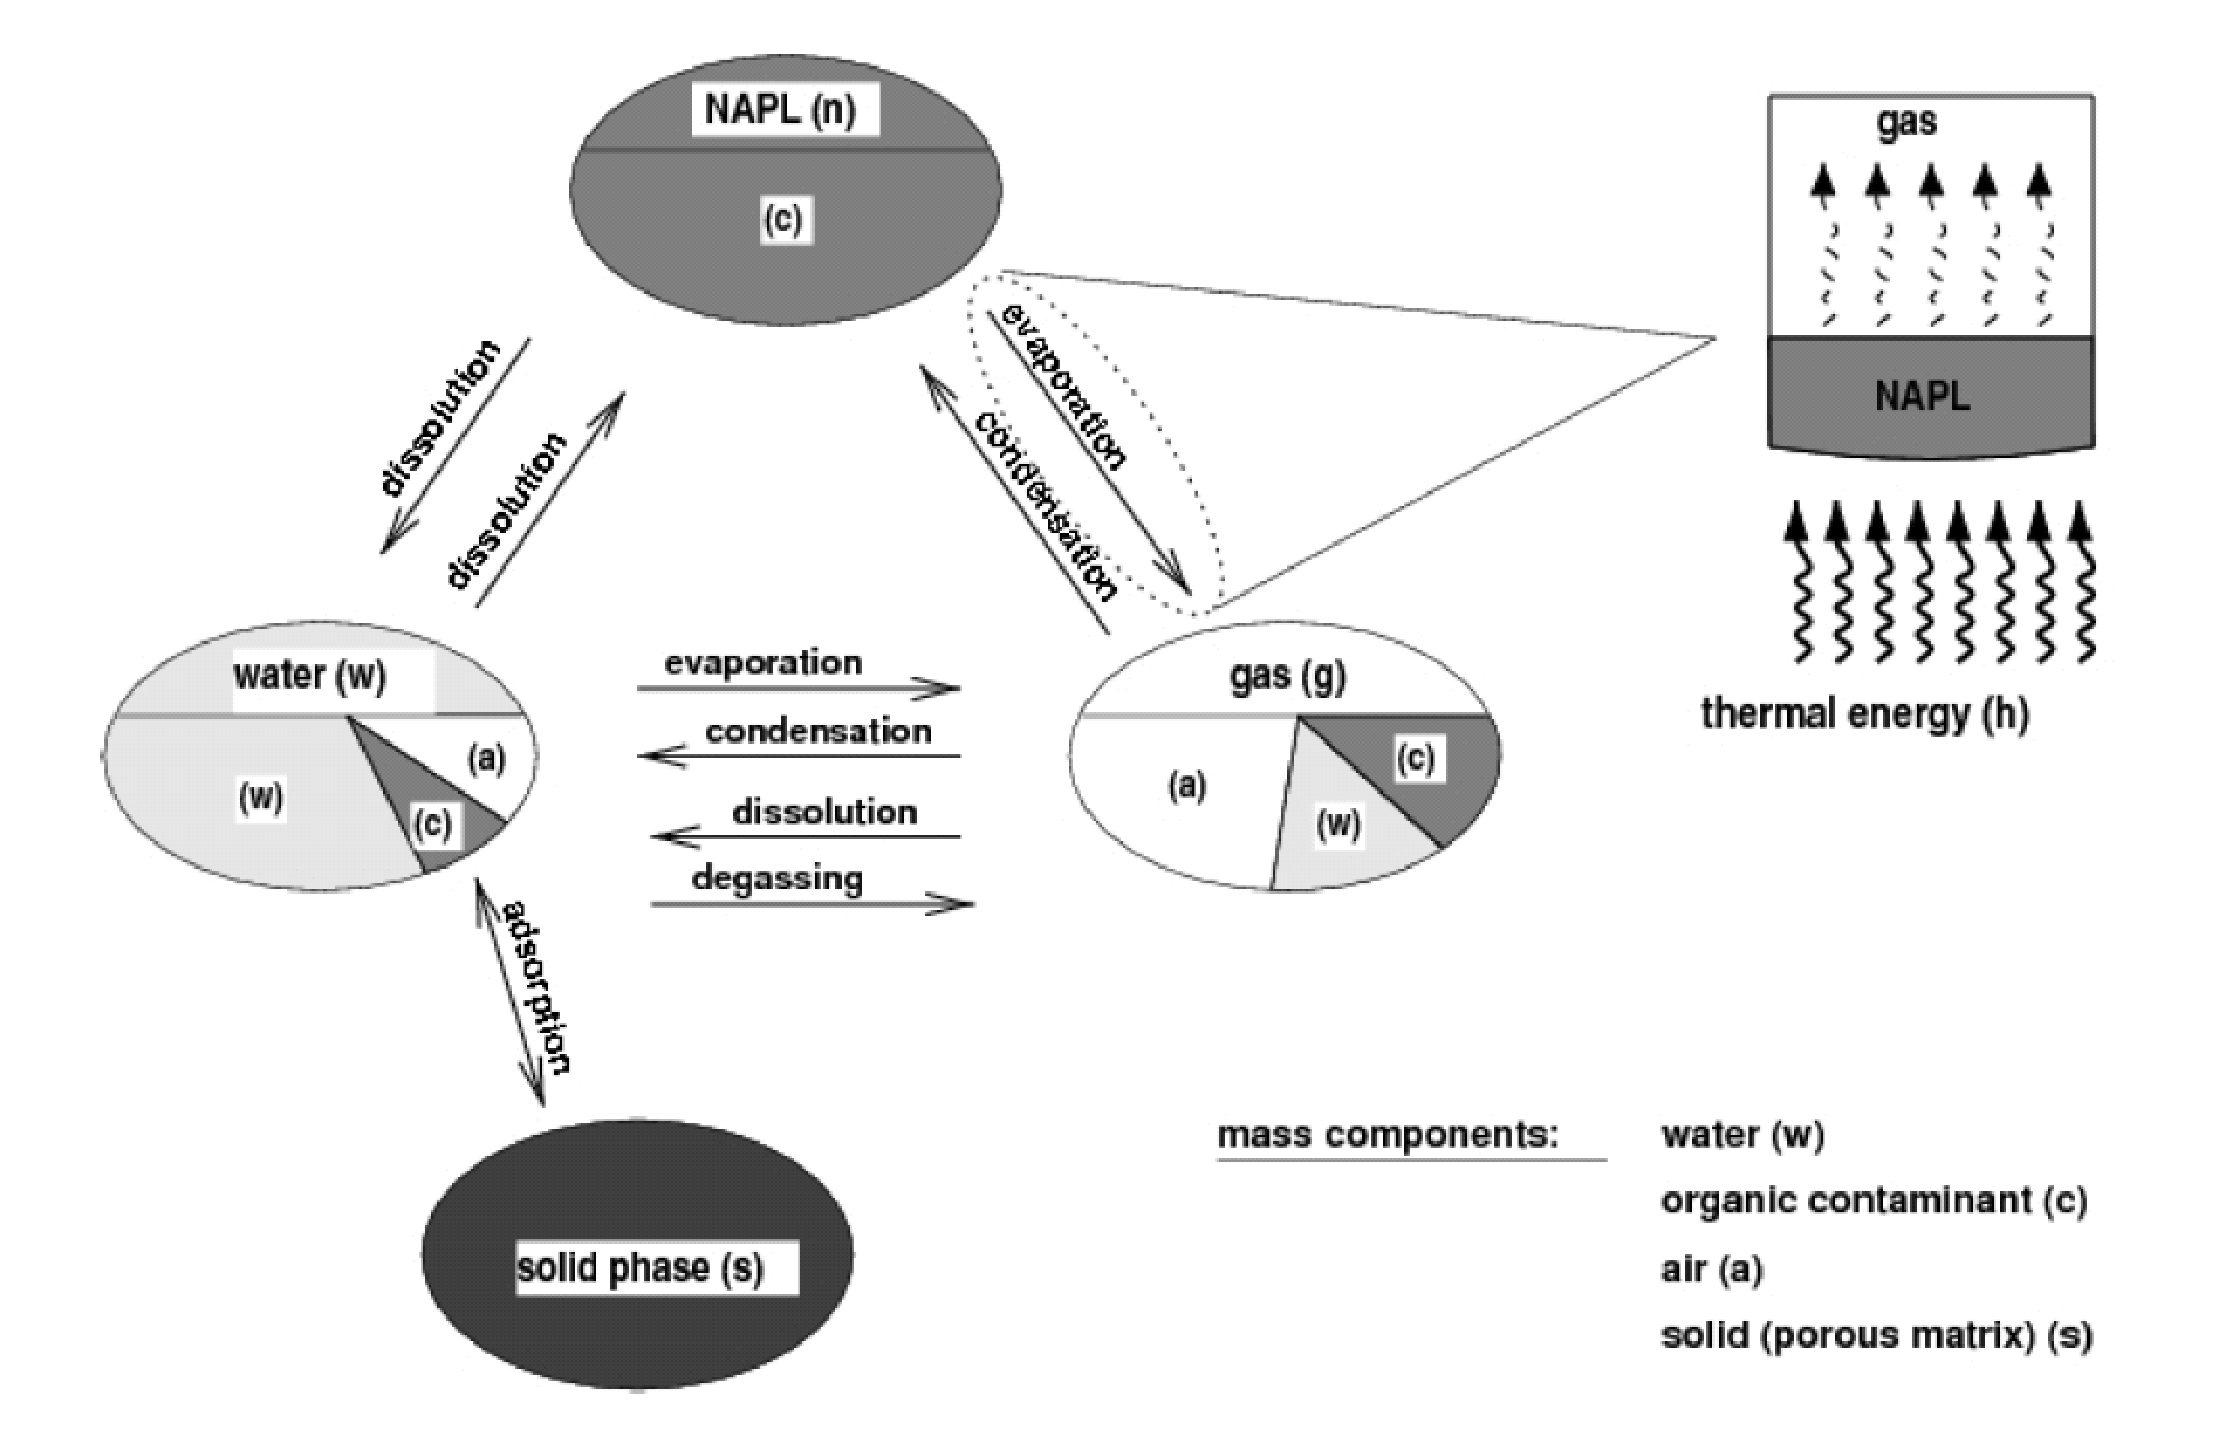
\includegraphics[width=0.7\linewidth]{EPS/masstransfer}
  \caption{Mass and energy transfer between the phases}
  \label{A3:fig:mundwtrans}
\end{figure}

\textbf{Equilibrium:}
For the nonisothermal multiphase processes in porous media under
consideration, we state that the assumption of local thermal
equilibrium is valid since flow velocities are small. We neglect
chemical reactions and biological decomposition and assume chemical
equilibrium.  Mechanical equilibrium is not valid in a porous medium, 
since discontinuities in pressure can occur across a fluid-fluid
interface due to capillary effects.

\textbf{Notation:} The index $\alpha \in \{\text{w}, \text{n}, \text{g}\}$ refers 
to the phase, while the superscript $\kappa \in \{\text{w}, \text{a}, \text{c}\}$ refers 
to the component. \\
\begin{tabular}{llll}
$p_\alpha$ & phase pressure & $\phi$ & porosity \\
$T$ & temperature & $K$ & absolute permeability tensor \\
$S_\alpha$ & phase saturation & $\tau$ & tortuosity \\
$x_\alpha^\kappa$ & mole fraction of component $\kappa$ in phase $\alpha$ & $\boldsymbol{g}$ & gravitational acceleration \\
$X_\alpha^\kappa$ & mass fraction of component $\kappa$ in phase $\alpha$ & $q^\kappa_\alpha$ & volume source term of $\kappa$ in $\alpha$ \\
$\varrho_{\text{mol},\alpha}$ & molar density of phase $\alpha$ & $u_\alpha$ & specific internal energy \\
$\varrho_{\alpha}$ & mass density of phase $\alpha$ & $h_\alpha$ & specific enthalpy \\
$k_{\text{r}\alpha}$ & relative permeability & $c_\text{s}$ & specific heat enthalpy \\
$\mu_\alpha$ & phase viscosity & $\lambda_\text{pm}$ & heat conductivity \\
$D_\alpha^\kappa$ & diffusivity of component $\kappa$ in phase $\alpha$ & $q^h$ & heat source term \\
$\boldsymbol{v}_\alpha$ & Darcy velocity & $\boldsymbol{v}_{a,\alpha}$  & advective velocity
\end{tabular}


\subsection{Balance Equations}
For the balance equations for multicomponent systems, it is in many
cases convenient to use a molar formulation of the continuity
equation. Considering the mass conservation for each component allows
us to drop source/sink terms for describing the mass transfer between
phases. Then, the
molar mass balance can be written as:
%
\begin{multline}
  \label{A3:eqmass1}
 \phi \frac{\partial (\sum_\alpha \varrho_{\text{mol}, \alpha}
    x_\alpha^\kappa S_\alpha )}{\partial t}  
 - \sum\limits_\alpha \Div \left( \frac{k_{\text{r}
        \alpha}}{\mu_\alpha} \varrho_{\text{mol}, \alpha}
    x_\alpha^\kappa K (\grad p_\alpha -
    \varrho_{\alpha} \boldsymbol{g}) \right)  \\
  % 
  %
 - \sum\limits_\alpha \Div \left( \tau \phi S_\alpha D_\alpha^\kappa \varrho_{\text{mol},
      \alpha} \grad x_\alpha^\kappa \right)  
 - q^\kappa = 0, \qquad \kappa \in \{\text{w,a,c}\}.
\end{multline}

The component mass balance can also be written in terms of mass fractions 
by replacing molar densities by mass densities and mole by mass fractions.
To obtain a single conserved quantity in the temporal derivative, the total 
concentration, representing the mass of one component per unit volume, is defined as
\begin{displaymath}
C^\kappa = \sum_\alpha \phi S_\alpha \varrho_{\text{mass},\alpha} X_\alpha^\kappa \; .
\end{displaymath}
Using this definition, the component mass balance is written as:

\begin{multline}
  \label{A3:eqmass2}
    \frac{\partial C^\kappa}{\partial t} = 
  \sum\limits_\alpha \Div \left( \frac{k_{\text{r}
        \alpha}}{\mu_\alpha} \varrho_{\text{mass}, \alpha}
    X_\alpha^\kappa K (\grad p_\alpha +
    \varrho_{\text{mass}, \alpha} \boldsymbol{g}) \right)  \\
  %
  %
   + \sum\limits_\alpha \Div \left( \tau \phi S_\alpha D_\alpha^\kappa \varrho_{\text{mass},
      \alpha} \grad X_\alpha^\kappa \right)  
 + q^\kappa = 0, \qquad \kappa \in \{\text{w,a,c}\}.
\end{multline}


In the case of non-isothermal systems, we further have to balance the
thermal energy. We assume fully reversible processes, such that entropy
is not needed as a model parameter. Furthermore, we neglect 
dissipative effects and the heat transport due to molecular
diffusion. The energy balance can then be
formulated as:
%
\begin{multline}
  \label{A3:eqenergmak1}
  \phi \frac{\partial \left( \sum_\alpha \varrho_{\alpha}
      u_\alpha S_\alpha \right)}{\partial t} + \left( 1 -
    \phi \right) \frac{\partial \varrho_{\text{s}} c_{\text{s}}
    T}{\partial t}  
 - \Div \left( \lambda_{\text{pm}} \grad T \right)
   \\
   - \sum\limits_\alpha \Div \left( \frac{k_{\text{r}
        \alpha}}{\mu_\alpha} \varrho_{\alpha} h_\alpha
    K \left( \grad p_\alpha - \varrho_{\alpha}
      \boldsymbol{g} \right) \right)  
 - q^h \; = \; 0.
\end{multline}

In order to close the system, supplementary constraints for capillary pressure, saturations and mole
fractions are needed, \cite{A3:helmig:1997}. 
According to the Gibbsian phase rule, the number of degrees of freedom
in a non-isothermal compositional multiphase system is equal to the
number of components plus one. This means we need as many independent
unknowns in the system description. The
available primary variables are, e.\ g., saturations, mole/mass
fractions, temperature, pressures, etc.

\section{Box method - A short introduction}\label{box}

For the spatial discretization the so called BOX-method is used which unites the advantages of the finite-volume (FV) and finite-element (FE) methods. 

First, the model domain $G$ is discretized with a FE mesh consisting of nodes i and corresponding elements $E_k$. Then, a secondary FV mesh is constructed by connecting the midpoints and barycenters of the elements surrounding node i creating a box $B_i$ around node i (see Figure \ref{pc:box}a). 

\begin{figure} [h]
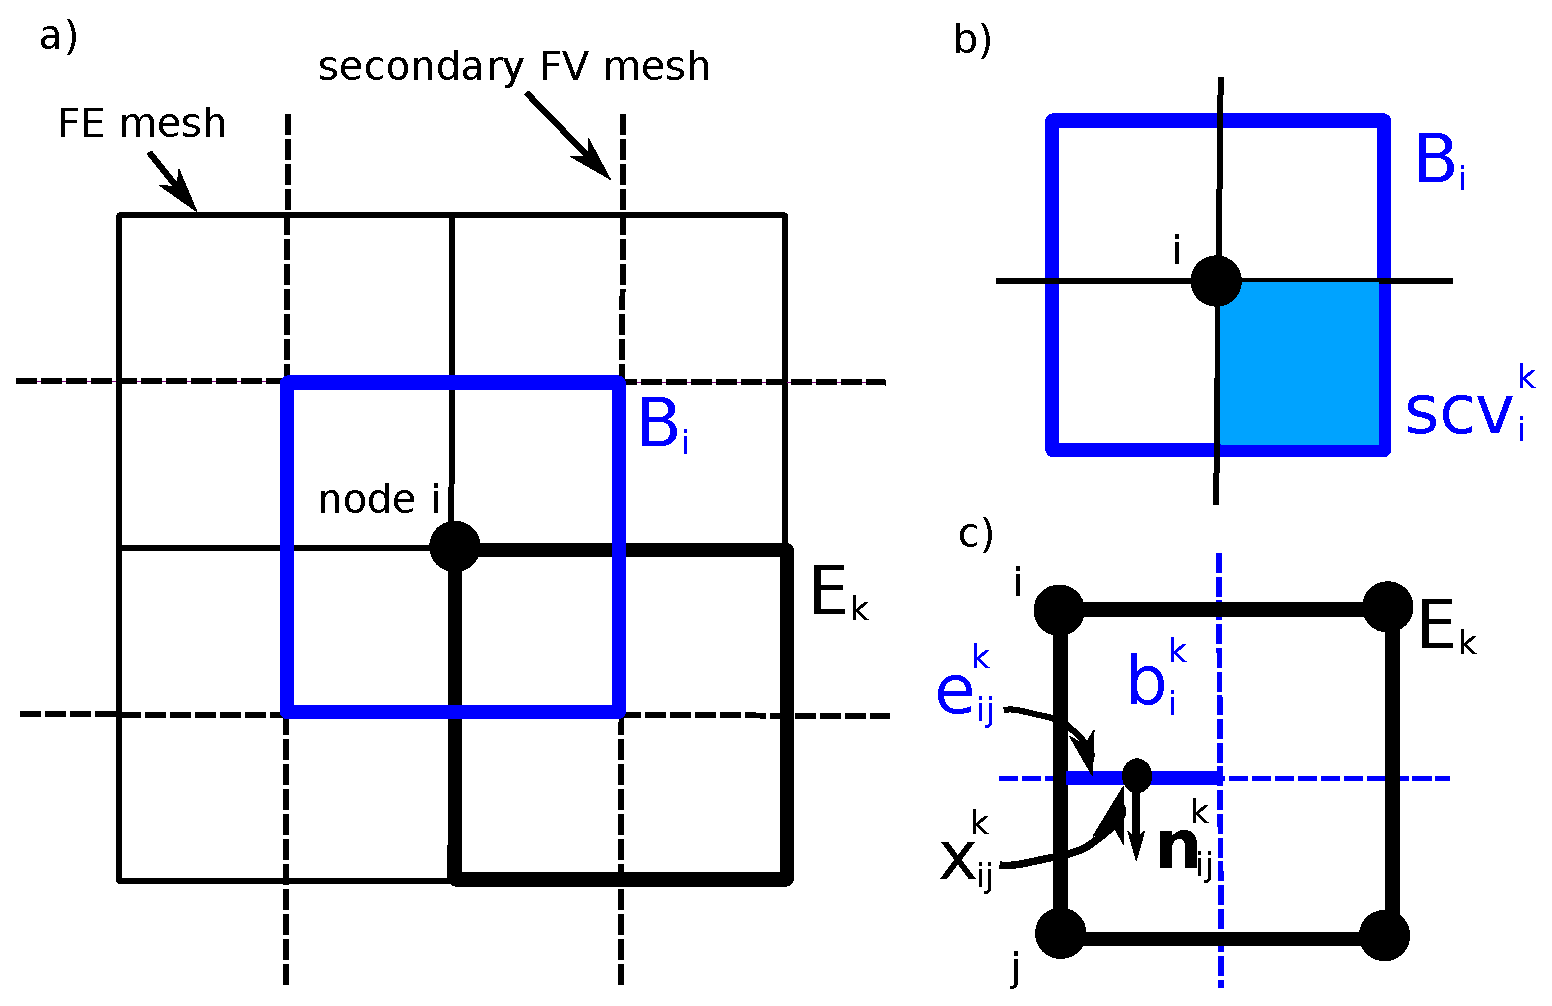
\includegraphics[width=0.8\linewidth,keepaspectratio]{EPS/box_disc}
\caption{\label{pc:box} Discretization of the BOX-method}
\end{figure}

The FE mesh divides the box $B_i$ into subcontrolvolumes (scv's) $b^k_i$ (see Figure \ref{pc:box}b). Figure \ref{pc:box}c shows the finite element $E_k$ and the scv's $b^k_i$ inside $E_k$, which belong to four different boxes $B_i$. Also necessary for the discretization are the faces of the subcontrolvolumes (scvf's) $e^k_{ij}$ between the scv's $b^k_i$ and $b^k_j$, where $|e^k_{ij}|$ is the length of the scvf. The integration points $x^k_{ij}$ on $e^k_{ij}$ and the outer normal vector $\mathbf n^k_{ij}$ are also to be defined (see Figure \ref{pc:box}c).

The advantage of the FE method is that unstructured grids can be used, while the FV method is mass conservative. The idea is to apply the FV method (balance of fluxes across the interfaces) to each FV box $B_i$  and to get the fluxes across the interfaces $e^k_{ij}$ at the integration points $x^k_{ij}$ from the FE approach. Consequently, at each scvf the following expression results:

\begin{equation}
 	f(\tilde u(x^k_{ij})) \cdot \mathbf n^k_{ij} \: |e^k_{ij}| \qquad \textrm{with} \qquad \tilde u(x^k_{ij}) = \sum_i N_i(x^k_{ij}) \cdot \hat u_i .
\end{equation}

In the following, the discretization of the balance equation is going to be derived. From the \textsc{Reynolds} transport theorem follows the general balance equation:

\begin{equation}
	\underbrace{\int_G \frac{\partial}{\partial t} \: u \: dG}_{1} + \underbrace{\int_{\partial G} (\mathbf{v} u + \mathbf w) \cdot \textbf n \: d\varGamma}_{2} = \underbrace{\int_G q \: dG}_{3}
\end{equation}

\begin{equation}
	f(u) = \int_G \frac{\partial u}{\partial t} \: dG + \int_{G} \nabla \cdot \underbrace{\left[  \mathbf{v} u + \mathbf w(u)\right] }_{F(u)}  \: dG - \int_G q \: dG = 0
\end{equation}
where term 1 describes the changes of entity $u$ within a control volume over time, term 2 the advective, diffusive and dispersive fluxes over the interfaces of the control volume and term 3 is the source and sink term. $G$ denotes the model domain and $F(u) = F(\mathbf v, p) = F(\mathbf v(x,t), p(x,t))$.

Like the FE method, the BOX-method follows the principle of weighted residuals. In the function $f(u)$ the unknown $u$ is approximated by discrete values at the nodes of the FE mesh $\hat u_i$ and linear basis functions $N_i$ yielding an approximate function $f(\tilde u)$. For $u\in \lbrace \mathbf v, p, x^\kappa \rbrace$ this means

\begin{minipage}[b]{0.47\textwidth}
\begin{equation}
\label{eq:p} 
	\tilde p = \sum_i N_i \hat{p_i}
\end{equation}
\begin{equation}
\label{eq:v} 
	\tilde{\mathbf v} = \sum_i N_i \hat{\mathbf v}
\end{equation}
\begin{equation}
\label{eq:x} 
	\tilde x^\kappa  = \sum_i N_i \hat x^\kappa 
\end{equation}
\end{minipage}
\hfill
\begin{minipage}[b]{0.47\textwidth}
\begin{equation}
\label{eq:dp} 
	\nabla \tilde p = \sum_i \nabla N_i \hat{p_i}
\end{equation}
\begin{equation}
\label{eq:dv} 
	\nabla \tilde{\mathbf v} = \sum_i \nabla N_i \hat{\mathbf v}
\end{equation}
\begin{equation}
\label{eq:dx} 
	\nabla \tilde x^\kappa  = \sum_i \nabla N_i \hat x^\kappa .
\end{equation}
\end{minipage} 

Due to the approximation with node values and basis functions the differential equations are not exactly fulfilled anymore but a residual $\varepsilon$ is produced.

\begin{equation}
	f(u) = 0  \qquad \Rightarrow \qquad f(\tilde u) = \varepsilon
\end{equation}

Application of the principle of weighted residuals, meaning the multiplication of the residual $\varepsilon$ with a weighting function $W_j$  and claiming that this product has to vanish within the whole domain,

\begin{equation}
	\int_G W_j \cdot \varepsilon \: \overset {!}{=} \: 0 \qquad \textrm{with} \qquad \sum_j W_j =1
\end{equation}
yields the following equation:

\begin{equation}
	\int_G W_j \frac{\partial \tilde u}{\partial t} \: dG + \int_G W_j \cdot \left[ \nabla \cdot F(\tilde u) \right]  \: dG - \int_G W_j \cdot q \: dG = \int_G W_j \cdot \varepsilon \: dG \: \overset {!}{=} \: 0 .
\end{equation}

Then, the chain rule and the \textsc{Green-Gaussian} integral theorem are applied.

\begin{equation}
	\int_G W_j \frac{\partial \sum_i N_i \hat u_i}{\partial t} \: dG + \int_{\partial G}  \left[ W_j \cdot F(\tilde u)\right]  \cdot \mathbf n \: d\varGamma_G + \int_G  \nabla W_j \cdot F(\tilde u)  \: dG - \int_G W_j \cdot q \: dG = 0
\end{equation}

A mass lumping technique is applied by assuming that the storage capacity is reduced to the nodes. This means that the integrals $M_{i,j} = \int_G W_j \: N_i \: dG$ are replaced by the mass lumping term $M^{lump}_{i,j}$ which is defined as:

\begin{equation}
	 M^{lump}_{i,j} =\begin{cases} \int_G W_j \: dG = \int_G N_i \: dG = V_i &i = j\\
	0 &i \neq j\\
	         \end{cases}
\end{equation}
where $V_i$ is the volume of the FV box $B_i$ associated with node i. The application of this assumption in combination with $\int_G W_j \:q \: dG = V_i \: q$ yields

\begin{equation}
	V_i \frac{\partial \hat u_i}{\partial t} + \int_{\partial G}  \left[ W_j \cdot F(\tilde u)\right]  \cdot \mathbf n \: d\varGamma_G + \int_G  \nabla W_j \cdot F(\tilde u)  \: dG- V_i \cdot q = 0 \, .
\end{equation}

Defining the weighting function $W_j$ to be piecewisely constant over a control volume box $B_i$ 

\begin{equation}
	W_j(x) = \begin{cases}
	          1 &x \in B_i \\
		  0 &x \notin B_i\\
	         \end{cases}
\end{equation}

causes $\nabla W_j = 0$:

\begin{equation}
\label{eq:disc1} 
	V_i \frac{\partial \hat u_i}{\partial t} + \int_{\partial B_i}  \left[ W_j \cdot F(\tilde u)\right] \cdot \mathbf n  \;  d{\varGamma}_{B_i} - V_i \cdot q = 0 .
\end{equation}

The consideration of the time discretization and inserting $W_j = 1$ finally lead to the discretized form which will be applied to the mathematical flow and transport equations:

\begin{equation}
\label{eq:discfin} 
	V_i \frac{\hat u_i^{n+1} - \hat u_i^{n}}{\Delta t} + \int_{\partial B_i}  F(\tilde u^{n+1}) \cdot \mathbf n  \;  d{\varGamma}_{B_i} - V_i \: q^{n+1} \: = 0 
\end{equation}



\section{Available models} 
The following description of the available models is automatically extracted 
from the Doxygen documentation.
% \textbf{TODO}: Unify notation. 

\subsection{Fully-implicit models} 

The fully-implicit models described in this section are using the box
scheme as described in Section \ref{box} for spatial and the implicit Euler
method as temporal discretization. The models themselves are located in
subdirectories of \texttt{ewoms/boxmodels} of the \eWoms distribution.

\subsubsection{The immiscible multi-phase model} 
%%%%%%%%%%%%%%%%%%%%%%%%%%%%%%%%%%%%%%%%%%%%%%%%%%%%%%%%%%%%%%%%%
% This file has been autogenerated from the LaTeX part of the   %
% doxygen documentation; DO NOT EDIT IT! Change the model's .hh %
% file instead!!                                                %
%%%%%%%%%%%%%%%%%%%%%%%%%%%%%%%%%%%%%%%%%%%%%%%%%%%%%%%%%%%%%%%%%

This model multi-\/phase flow of $M > 0$ immiscible fluids $\alpha$. By default, the standard multi-\/phase Darcy approach is used to determine the velocity, i.\-e. \[ \mathbf{v}_\alpha = - \frac{k_{r\alpha}}{\mu_\alpha} \mathbf{K} \left(\text{grad}\, p_\alpha - \varrho_{\alpha} \mathbf{g} \right) \;, \] although the actual approach which is used can be specified via the {\ttfamily Velocity\-Module} property. For example, the velocity model can by changed to the Forchheimer approach by
\begin{lstlisting}[style=eWomsCode]
 SET_TYPE_PROP(MyProblemTypeTag, VelocityModule,
      Ewoms::BoxForchheimerVelocityModule<TypeTag>);
\end{lstlisting}


The core of the model is the conservation mass of each component by means of the equation \[ \frac{\partial\;\phi S_\alpha \rho_\alpha }{\partial t} - \text{div} \left\{ \rho_\alpha \mathbf{v}_\alpha \right\} - q_\alpha = 0 \;. \]

These equations are discretized by a fully-\/coupled vertex centered finite volume (box) scheme as spatial and the implicit Euler method as time discretization.

The model uses the following primary variables\-:
\begin{itemize}
\item The pressure $p_0$ in Pascal of the phase with the lowest index
\item The saturations $S_\alpha$ of the $M - 1$ phases that exhibit the lowest indices
\item The absolute temperature $T$ in Kelvin if energy is conserved via the energy equation
\end{itemize}



\subsubsection{The miscible multi-phase NCP model} 
%%%%%%%%%%%%%%%%%%%%%%%%%%%%%%%%%%%%%%%%%%%%%%%%%%%%%%%%%%%%%%%%%
% This file has been autogenerated from the LaTeX part of the   %
% doxygen documentation; DO NOT EDIT IT! Change the model's .hh %
% file instead!!                                                %
%%%%%%%%%%%%%%%%%%%%%%%%%%%%%%%%%%%%%%%%%%%%%%%%%%%%%%%%%%%%%%%%%

This model assumes a flow of $M \geq 1$ fluid phases $\alpha$, each of which is assumed to be a mixture $N \geq M$ chemical species $\kappa$.

By default, the standard multi-\/phase Darcy approach is used to determine the velocity, i.\-e. \[ \mathbf{v}_\alpha = - \frac{k_{r\alpha}}{\mu_\alpha} \mathbf{K} \left(\text{grad}\, p_\alpha - \varrho_{\alpha} \mathbf{g} \right) \;, \] although the actual approach which is used can be specified via the {\ttfamily Velocity\-Module} property. For example, the velocity model can by changed to the Forchheimer approach by
\begin{lstlisting}[style=eWomsCode]
 SET_TYPE_PROP(MyProblemTypeTag, VelocityModule,
      Dumux::BoxForchheimerVelocityModule<TypeTag>);
\end{lstlisting}


The core of the model is the conservation mass of each component by means of the equation \[ \sum_\alpha \frac{\partial\;\phi c_\alpha^\kappa S_\alpha }{\partial t} - \sum_\alpha \text{div} \left\{ c_\alpha^\kappa \mathbf{v}_\alpha \right\} - q^\kappa = 0 \;. \]

To close the system mathematically, $M$ model equations are also required. This model uses the primary variable switching assumptions, which are given by\-: \[ 0 \stackrel{!}{=} f_\alpha = \left\{ \begin{array}{cl} S_\alpha & \quad \text{if phase }\alpha\text{ is not present} \\ 1 - \sum_\kappa x_\alpha^\kappa & \quad \text{else} \end{array} \right. \]

To make this approach applicable, a pseudo primary variable {\itshape phase presence} has to be introduced. Its purpose is to specify for each phase whether it is present or not. It is a {\itshape pseudo} primary variable because it is not directly considered when linearizing the system in the Newton method, but after each Newton iteration, it gets updated like the \char`\"{}real\char`\"{} primary variables. The following rules are used for this update procedure\-:


\begin{itemize}
\item If phase $\alpha$ is present according to the pseudo primary variable, but $S_\alpha < 0$ after the Newton update, consider the phase $\alpha$ disappeared for the next iteration and use the set of primary variables which correspond to the new phase presence.


\item If phase $\alpha$ is not present according to the pseudo primary variable, but the sum of the component mole fractions in the phase is larger than 1, i.\-e. $\sum_\kappa x_\alpha^\kappa > 1$, consider the phase $\alpha$ present in the the next iteration and update the set of primary variables to make it consistent with the new phase presence.


\item In all other cases don't modify the phase presence for phase $\alpha$.


\end{itemize}

The model always requires $N$ primary variables, but their interpretation is dependent on the phase presence\-:


\begin{itemize}
\item The first primary variable is always interpreted as the pressure of the phase with the lowest index $PV_0 = p_0$.


\item Then, $M - 1$ \char`\"{}switching primary variables\char`\"{} follow, which are interpreted depending in the presence of the first $M-1$ phases\-: If phase $\alpha$ is present, its saturation $S_\alpha = PV_i$ is used as primary variable; if it is not present, the mole fraction $PV_i = x_{\alpha^\star}^\alpha$ of the component with index $\alpha$ in the phase with the lowest index that is present $\alpha^\star$ is used instead.


\item Finally, the mole fractions of the $N-M$ components with the largest index in the phase with the lowest index that is present $x_{\alpha^\star}^\kappa$ are used as primary variables.


\end{itemize}

This model is then discretized using a fully-\/coupled vertex centered finite volume (box) scheme as spatial and the implicit Euler method as temporal discretization.



\subsubsection{The miscible multi-phase PVS model} 
%%%%%%%%%%%%%%%%%%%%%%%%%%%%%%%%%%%%%%%%%%%%%%%%%%%%%%%%%%%%%%%%%
% This file has been autogenerated from the LaTeX part of the   %
% doxygen documentation; DO NOT EDIT IT! Change the model's .hh %
% file instead!!                                                %
%%%%%%%%%%%%%%%%%%%%%%%%%%%%%%%%%%%%%%%%%%%%%%%%%%%%%%%%%%%%%%%%%

This model assumes a flow of $M \geq 1$ fluid phases $\alpha$, each of which is assumed to be a mixture $N \geq M$ chemical species $\kappa$.

By default, the standard multi-\/phase Darcy approach is used to determine the velocity, i.\-e. \[ \mathbf{v}_\alpha = - \frac{k_{r\alpha}}{\mu_\alpha} \mathbf{K} \left(\text{grad}\, p_\alpha - \varrho_{\alpha} \mathbf{g} \right) \;, \] although the actual approach which is used can be specified via the {\ttfamily Velocity\-Module} property. For example, the velocity model can by changed to the Forchheimer approach by
\begin{lstlisting}[style=eWomsCode]
 SET_TYPE_PROP(MyProblemTypeTag, VelocityModule,
      Dumux::BoxForchheimerVelocityModule<TypeTag>);
\end{lstlisting}


The core of the model is the conservation mass of each component by means of the equation \[ \sum_\alpha \frac{\partial\;\phi c_\alpha^\kappa S_\alpha }{\partial t} - \sum_\alpha \text{div} \left\{ c_\alpha^\kappa \mathbf{v}_\alpha \right\} - q^\kappa = 0 \;. \]

To close the system mathematically, $M$ model equations are also required. This model uses the primary variable switching assumptions, which are given by\-: \[ 0 \stackrel{!}{=} f_\alpha = \left\{ \begin{array}{cl} S_\alpha & \quad \text{if phase }\alpha\text{ is not present} \\ 1 - \sum_\kappa x_\alpha^\kappa & \quad \text{else} \end{array} \right. \]

To make this approach applicable, a pseudo primary variable {\itshape phase presence} has to be introduced. Its purpose is to specify for each phase whether it is present or not. It is a {\itshape pseudo} primary variable because it is not directly considered when linearizing the system in the Newton method, but after each Newton iteration, it gets updated like the \char`\"{}real\char`\"{} primary variables. The following rules are used for this update procedure\-:


\begin{itemize}
\item If phase $\alpha$ is present according to the pseudo primary variable, but $S_\alpha < 0$ after the Newton update, consider the phase $\alpha$ disappeared for the next iteration and use the set of primary variables which correspond to the new phase presence.


\item If phase $\alpha$ is not present according to the pseudo primary variable, but the sum of the component mole fractions in the phase is larger than 1, i.\-e. $\sum_\kappa x_\alpha^\kappa > 1$, consider the phase $\alpha$ present in the the next iteration and update the set of primary variables to make it consistent with the new phase presence.


\item In all other cases don't modify the phase presence for phase $\alpha$.


\end{itemize}

The model always requires $N$ primary variables, but their interpretation is dependent on the phase presence\-:


\begin{itemize}
\item The first primary variable is always interpreted as the pressure of the phase with the lowest index $PV_0 = p_0$.


\item Then, $M - 1$ \char`\"{}switching primary variables\char`\"{} follow, which are interpreted depending in the presence of the first $M-1$ phases\-: If phase $\alpha$ is present, its saturation $S_\alpha = PV_i$ is used as primary variable; if it is not present, the mole fraction $PV_i = x_{\alpha^\star}^\alpha$ of the component with index $\alpha$ in the phase with the lowest index that is present $\alpha^\star$ is used instead.


\item Finally, the mole fractions of the $N-M$ components with the largest index in the phase with the lowest index that is present $x_{\alpha^\star}^\kappa$ are used as primary variables.


\end{itemize}

This model is then discretized using a fully-\/coupled vertex centered finite volume (box) scheme as spatial and the implicit Euler method as temporal discretization.



\subsubsection{The miscible multi-phase flash model} 
%%%%%%%%%%%%%%%%%%%%%%%%%%%%%%%%%%%%%%%%%%%%%%%%%%%%%%%%%%%%%%%%%
% This file has been autogenerated from the LaTeX part of the   %
% doxygen documentation; DO NOT EDIT IT! Change the model's .hh %
% file instead!!                                                %
%%%%%%%%%%%%%%%%%%%%%%%%%%%%%%%%%%%%%%%%%%%%%%%%%%%%%%%%%%%%%%%%%

A generic compositional multi-\/phase model using primary-\/variable switching.

This model assumes a flow of $M \geq 1$ fluid phases $\alpha$, each of which is assumed to be a mixture $N \geq M$ chemical species (denoted by the upper index $\kappa$).

By default, the standard multi-\/phase Darcy approach is used to determine the velocity, i.\-e. \[ \mathbf{v}_\alpha = - \frac{k_{r\alpha}}{\mu_\alpha} \mathbf{K} \left(\text{grad}\, p_\alpha - \varrho_{\alpha} \mathbf{g} \right) \;, \] although the actual approach which is used can be specified via the {\ttfamily Velocity\-Module} property. For example, the velocity model can by changed to the Forchheimer approach by
\begin{lstlisting}[style=eWomsCode]
 SET_TYPE_PROP(MyProblemTypeTag, VelocityModule,
      Dumux::BoxForchheimerVelocityModule<TypeTag>);
\end{lstlisting}


The core of the model is the conservation mass of each component by means of the equation \[ \sum_\alpha \frac{\partial\;\phi c_\alpha^\kappa S_\alpha }{\partial t} - \sum_\alpha \text{div} \left\{ c_\alpha^\kappa \mathbf{v}_\alpha \right\} - q^\kappa = 0 \;. \]

To determine the quanties that occur in the equations above, this model uses {\itshape flash calculations}. A flash solver starts with the total mass or molar mass per volume for each component and, calculates the compositions, saturations and pressures of all phases at a given temperature. For this the flash solver has to use some model assumptions internally. (Often these are the same primary variable switching or N\-C\-P assumptions as used by the other fully implicit compositional multi-\/phase models provided by e\-Woms.)

Using flash calculations for the flow model has some disadvantages\-:
\begin{itemize}
\item The accuracy of the flash solver needs to be sufficient to calculate the parital derivatives using numerical differentiation which are required for the Newton scheme.
\item Flash calculations tend to be quite computationally expensive and are often numerically unstable.
\end{itemize}

It is thus adviced to increase the target tolerance of the Newton scheme or a to use type for scalar values which exhibits higher precision than the standard {\ttfamily double} (e.\-g. {\ttfamily quad}) if this model ought to be used.

The model uses the following primary variables\-:
\begin{itemize}
\item The total molar concentration of each component\-: $c^\kappa = \sum_\alpha S_\alpha x_\alpha^\kappa \rho_{mol, \alpha}$
\item The absolute temperature \$\-T\$ in Kelvins if the energy equation enabled.
\end{itemize}



\subsubsection{The Richards model} 
%%%%%%%%%%%%%%%%%%%%%%%%%%%%%%%%%%%%%%%%%%%%%%%%%%%%%%%%%%%%%%%%%
% This file has been autogenerated from the LaTeX part of the   %
% doxygen documentation; DO NOT EDIT IT! Change the model's .hh %
% file instead!!                                                %
%%%%%%%%%%%%%%%%%%%%%%%%%%%%%%%%%%%%%%%%%%%%%%%%%%%%%%%%%%%%%%%%%

In the unsaturated zone, Richards' equation is frequently used to approximate the water distribution above the groundwater level. It can be derived from the two-\/phase equations, i.\-e. \[ \frac{\partial\;\phi S_\alpha \rho_\alpha}{\partial t} - \text{div} \left\{ \rho_\alpha \frac{k_{r\alpha}}{\mu_\alpha}\; \mathbf{K}\; \textbf{grad}\left[ p_\alpha - g\rho_\alpha \right] \right\} = q_\alpha, \] where $\alpha \in \{w, n\}$ is the index of the fluid phase, $\rho_\alpha$ is the fluid density, $S_\alpha$ is the fluid saturation, $\phi$ is the porosity of the soil, $k_{r\alpha}$ is the relative permeability for the fluid, $\mu_\alpha$ is the fluid's dynamic viscosity, $\mathbf{K}$ is the intrinsic permeability tensor, $p_\alpha$ is the fluid phase pressure and $g$ is the potential of the gravity field.

In contrast to the \char`\"{}full\char`\"{} two-\/phase model, the Richards model assumes that the non-\/wetting fluid is gas and that it thus exhibits a much lower viscosity than the (liquid) wetting phase. (This assumption is quite realistic in many applications\-: For example, at atmospheric pressure and at room temperature, the viscosity of air is only about $1\%$ of the viscosity of liquid water.) As a consequence, the $\frac{k_{r\alpha}}{\mu_\alpha}$ term typically is much larger for the gas phase than for the wetting phase. Using this reasoning, the Richards model assumes that $\frac{k_{rn}}{\mu_n}$ is infinitely large compared to the same term of the liquid phase. This implies that the pressure of the gas phase is equivalent to the static pressure distribution and that therefore, mass conservation only needs to be considered for the liquid phase.

The model thus choses the absolute pressure of the wetting phase $p_w$ as its only primary variable. The wetting phase saturation is calculated using the inverse of the capillary pressure, i.\-e. \[ S_w = p_c^{-1}(p_n - p_w) \] holds, where $p_n$ is a reference pressure given by the problem's {\ttfamily reference\-Pressure()} method. Nota bene, that the last step assumes that the capillary pressure-\/saturation curve can be uniquely inverted, i.\-e. it is not possible to set the capillary pressure to zero if the Richards model ought to be used!



\subsubsection{The black-oil model} 
%%%%%%%%%%%%%%%%%%%%%%%%%%%%%%%%%%%%%%%%%%%%%%%%%%%%%%%%%%%%%%%%%
% This file has been autogenerated from the LaTeX part of the   %
% doxygen documentation; DO NOT EDIT IT! Change the model's .hh %
% file instead!!                                                %
%%%%%%%%%%%%%%%%%%%%%%%%%%%%%%%%%%%%%%%%%%%%%%%%%%%%%%%%%%%%%%%%%

The black-\/oil model is a three-\/phase, three-\/component model widely used for oil reservoir simulation. The phases are denoted by lower index $\alpha \in \{ w, g, o \}$ (\char`\"{}water\char`\"{}, \char`\"{}gas\char`\"{} and \char`\"{}oil\char`\"{}) and the components by upper index $\kappa \in \{ W, G, O \}$ (\char`\"{}\-Water\char`\"{}, \char`\"{}\-Gas\char`\"{} and \char`\"{}\-Oil\char`\"{}). The model assumes partial miscibility\-:


\begin{itemize}
\item Water and the gas phases are immisicible and are assumed to be only composed of the water and gas components respectively-\/
\item The oil phase is assumed to be a mixture of the gas and the oil components.
\end{itemize}

The densities of the phases are determined by so-\/called {\itshape formation volume factors}\-:

\[ B_\alpha := \frac{\varrho_\alpha(1\,\text{bar})}{\varrho_\alpha(p_\alpha)} \]

Since the gas and water phases are assumed to be immiscible, this is sufficint to calculate their density. For the formation volume factor of the the oil phase $B_o$ determines the density of {\itshape saturated} oil, i.\-e. the density of the oil phase if some gas phase is present.

The composition of the oil phase is given by the {\itshape gas formation factor} $R_s$, which defined as the volume of gas at atmospheric pressure that is dissolved in saturated oil at a given pressure\-:

\[ R_s := \frac{x_o^G(p)\,\varrho_{mol,o}(p)}{\varrho_g(1\,\text{bar})}\;. \]

This allows to calculate all quantities required for the mass-\/conservation equations for each component, i.\-e.

\[ \sum_\alpha \frac{\partial\;\phi c_\alpha^\kappa S_\alpha }{\partial t} - \sum_\alpha \text{div} \left\{ c_\alpha^\kappa \mathbf{v}_\alpha \right\} - q^\kappa = 0 \;, \] where $\mathrm{v}_\alpha$ is the filter velocity of the phase $\alpha$.

By default $\mathrm{v}_\alpha$ is determined by using the standard multi-\/phase Darcy approach, i.\-e. \[ \mathbf{v}_\alpha = - \frac{k_{r\alpha}}{\mu_\alpha} \mathbf{K} \left(\text{grad}\, p_\alpha - \varrho_{\alpha} \mathbf{g} \right) \;, \] although the actual approach which is used can be specified via the {\ttfamily Velocity\-Module} property. For example, the velocity model can by changed to the Forchheimer approach by
\begin{lstlisting}[style=eWomsCode]
 SET_TYPE_PROP(MyProblemTypeTag, VelocityModule,
      Dumux::BoxForchheimerVelocityModule<TypeTag>);
\end{lstlisting}


The primary variables used by this model are\-:
\begin{itemize}
\item The pressure of the phase with the lowest index
\item The two saturations of the phases with the lowest indices
\end{itemize}



\subsubsection{The (Navier-)Stokes model} 
%%%%%%%%%%%%%%%%%%%%%%%%%%%%%%%%%%%%%%%%%%%%%%%%%%%%%%%%%%%%%%%%%
% This file has been autogenerated from the LaTeX part of the   %
% doxygen documentation; DO NOT EDIT IT! Change the model's .hh %
% file instead!!                                                %
%%%%%%%%%%%%%%%%%%%%%%%%%%%%%%%%%%%%%%%%%%%%%%%%%%%%%%%%%%%%%%%%%

This model implements Navier-\/\-Stokes flow of a single fluid. By default, it solves the momentum balance of the time-\/dependent Stokes equations, i.\-e. \[ \frac{\partial \left(\varrho\,\mathbf{v}\right)}{\partial t} + \boldsymbol{\nabla} p - \nabla \cdot \left( \mu \left(\boldsymbol{\nabla} \mathbf{v} + \boldsymbol{\nabla} \mathbf{v}^T\right) \right) - \varrho\,\mathbf{g} = 0\;, \] and the mass balance equation \[ \frac{\partial \varrho}{\partial t} + \nabla \cdot\left(\varrho\,\mathbf{v}\right) - q = 0 \;. \]

If the property {\ttfamily Enable\-Navier\-Stokes} is set to {\ttfamily true}, an additional convective momentum flux term (Navier term) gets included into the momentum conservation equations which allows to capture turbolent flow regimes. This additional term is given by \[ \varrho \left(\mathbf{v} \cdot \boldsymbol{\nabla} \right) \mathbf{v} \;. \]

These equations are discretized by a fully-\/coupled vertex-\/centered finite volume (box) scheme in space and using the implicit Euler method in time. Be aware, that this discretization scheme is quite unstable for the Navier-\/\-Stokes equations and quickly leads to unphysical oscillations in the calculated solution. We intend to use a more appropriate discretization scheme in the future, though.



%%% Local Variables: 
%%% mode: latex
%%% TeX-master: "ewoms-handbook"
%%% End: 
